%% The following is a directive for TeXShop to indicate the main file
%%!TEX root =../diss.tex

\chapter{Introduction}
\label{ch:Introduction}

Cancer is a disease that can occur at any age but mostly affects Canadians fifty years and older.
Based on estimates from 2010, 49\% of men and 45\% of women are expected to develop a type of cancer during their lifetimes and one in four Canadians are expected to die from cancer-related diseases~\cite{CancerSociety:2018tv}.
One approach to achieving better patient outcomes and reducing toxicity in cancer patients is to improve our understanding of tumour progression and treatment in preclinical tumour models using biological markers, also called biomarkers.
In 2001, the National Institutes of Health commissioned a working group to create standards and definitions for what would constitute an effective biomarker. 
A biomarker is ``a characteristic that is objectively measured and evaluated as an indicator of normal biological processes, pathogenic processes, or pharmacologic responses to a therapeutic intervention''~\cite{BiomarkersDefinitionsWorkingGroup:2001gd}.  
There is an urgent need for the development of new imaging biomarkers to aid in the development of more targeted tumour therapies~\cite{vanderMeel:2010cb}.
There has been considerable interest in the potential of predictive biomarkers for early assessment of tumour therapies. 
In this thesis, we aim to develop imaging-based biomarkers to explore the tumour microenvironment.

\section{Cancer biomarkers and targets} 

Hanahan and Weinberg catalogued a vast array of factors that contribute to tumour growth and provided a framework for understanding of diseases that result in abnormal cell growth~\cite{Hanahan:2000wo,Hanahan:2011gu}.
These ``hallmarks of cancer'' are ``essential alterations in cell physiology that collectively dictate malignant growth in tumours''~\cite{Hanahan:2000wo}.
These hallmarks are summarized in Fig.~\ref{cancerHallmarks} and the  work presented in this thesis focuses on the 5th hallmark, angiogenesis - the process by which new blood vessels form.

\begin{figure}[htbp]   
 \begin{center}  
 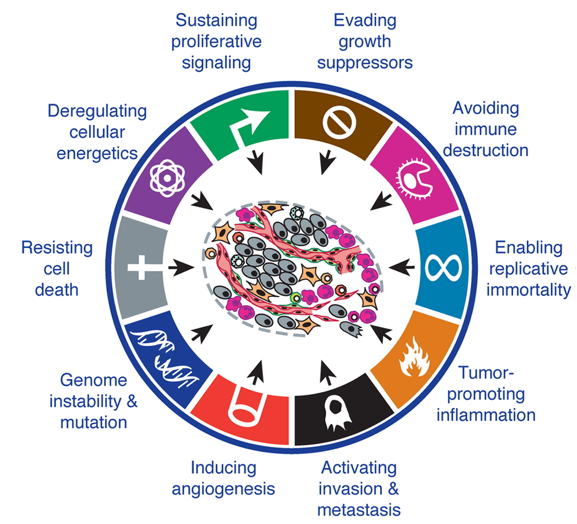
\includegraphics[width=4in]{intro/./intro-images/cancerHallmarks.png}
 \caption{Graphical illustration of the hallmarks of cancer as presented by Hanahan and Weinberg~\cite{Hanahan:2011gu}. Many of the targets described are inaccessible to non-invasive imaging and in this thesis, we focus on angiogenesis as the target of our imaging methods. Figure used with permission from Elsevier Inc.}  
 \label{cancerHallmarks}  
 \end{center}
\end{figure}

Angiogenesis is the formation of new blood vessels from pre-existing ones is a normal and vital process in the body tightly regulated by various cell signalling pathways and growth factors.
In tumours, angiogenesis is a critical step in the growth and spread of tumours as new blood vessels are recruited from the existing vascular network to promote rapidly accelerated and abnormal tumour growth~\cite{Folkman:1990ud}.
Normally, this process is regulated by several angiogenic and antiangiogenic factors such as $\alpha \beta$ integrin, vascular endothelial growth factor (\acs{VEGF}) and fibroblast growth factor~\cite{Laking:2006ij}.
In tumours however, this process is deregulated (Fig.~\ref{tumourVasculature}) and excess production of growth factors from rapidly proliferating tumour cells leads to a drastic increase in angiogenesis.
These newly formed vessels are unstable growth patterns of blood vessels in tumours are often described as abnormal with a defective and leaky endothelium~\cite{McDonald:2002ut}.
Irregular diameters of tumour vessels, abnormal branching patterns and leaky vessel walls all contribute to an increase in vessel permeability.
It is estimated that a single hole larger than 0.5$\mu$m in diameter would alter the permeability of that vessel significantly enough to result in solute extravasation to be limited by blood flow~\cite{McDonald:2002ut}.
Disorganized and inefficient blood flow also limits the delivery of macromolecules, such as chemotherapeutic agents via the blood.
Poor perfusion in the tumour due to a disorganized vascular network impairs the delivery of systemic drugs to the whole tumour and ultimately, reduces efficacy.

%\begin{wrapfigure}{L}{0.65\textwidth} 
\begin{figure}  
 \begin{center}  
 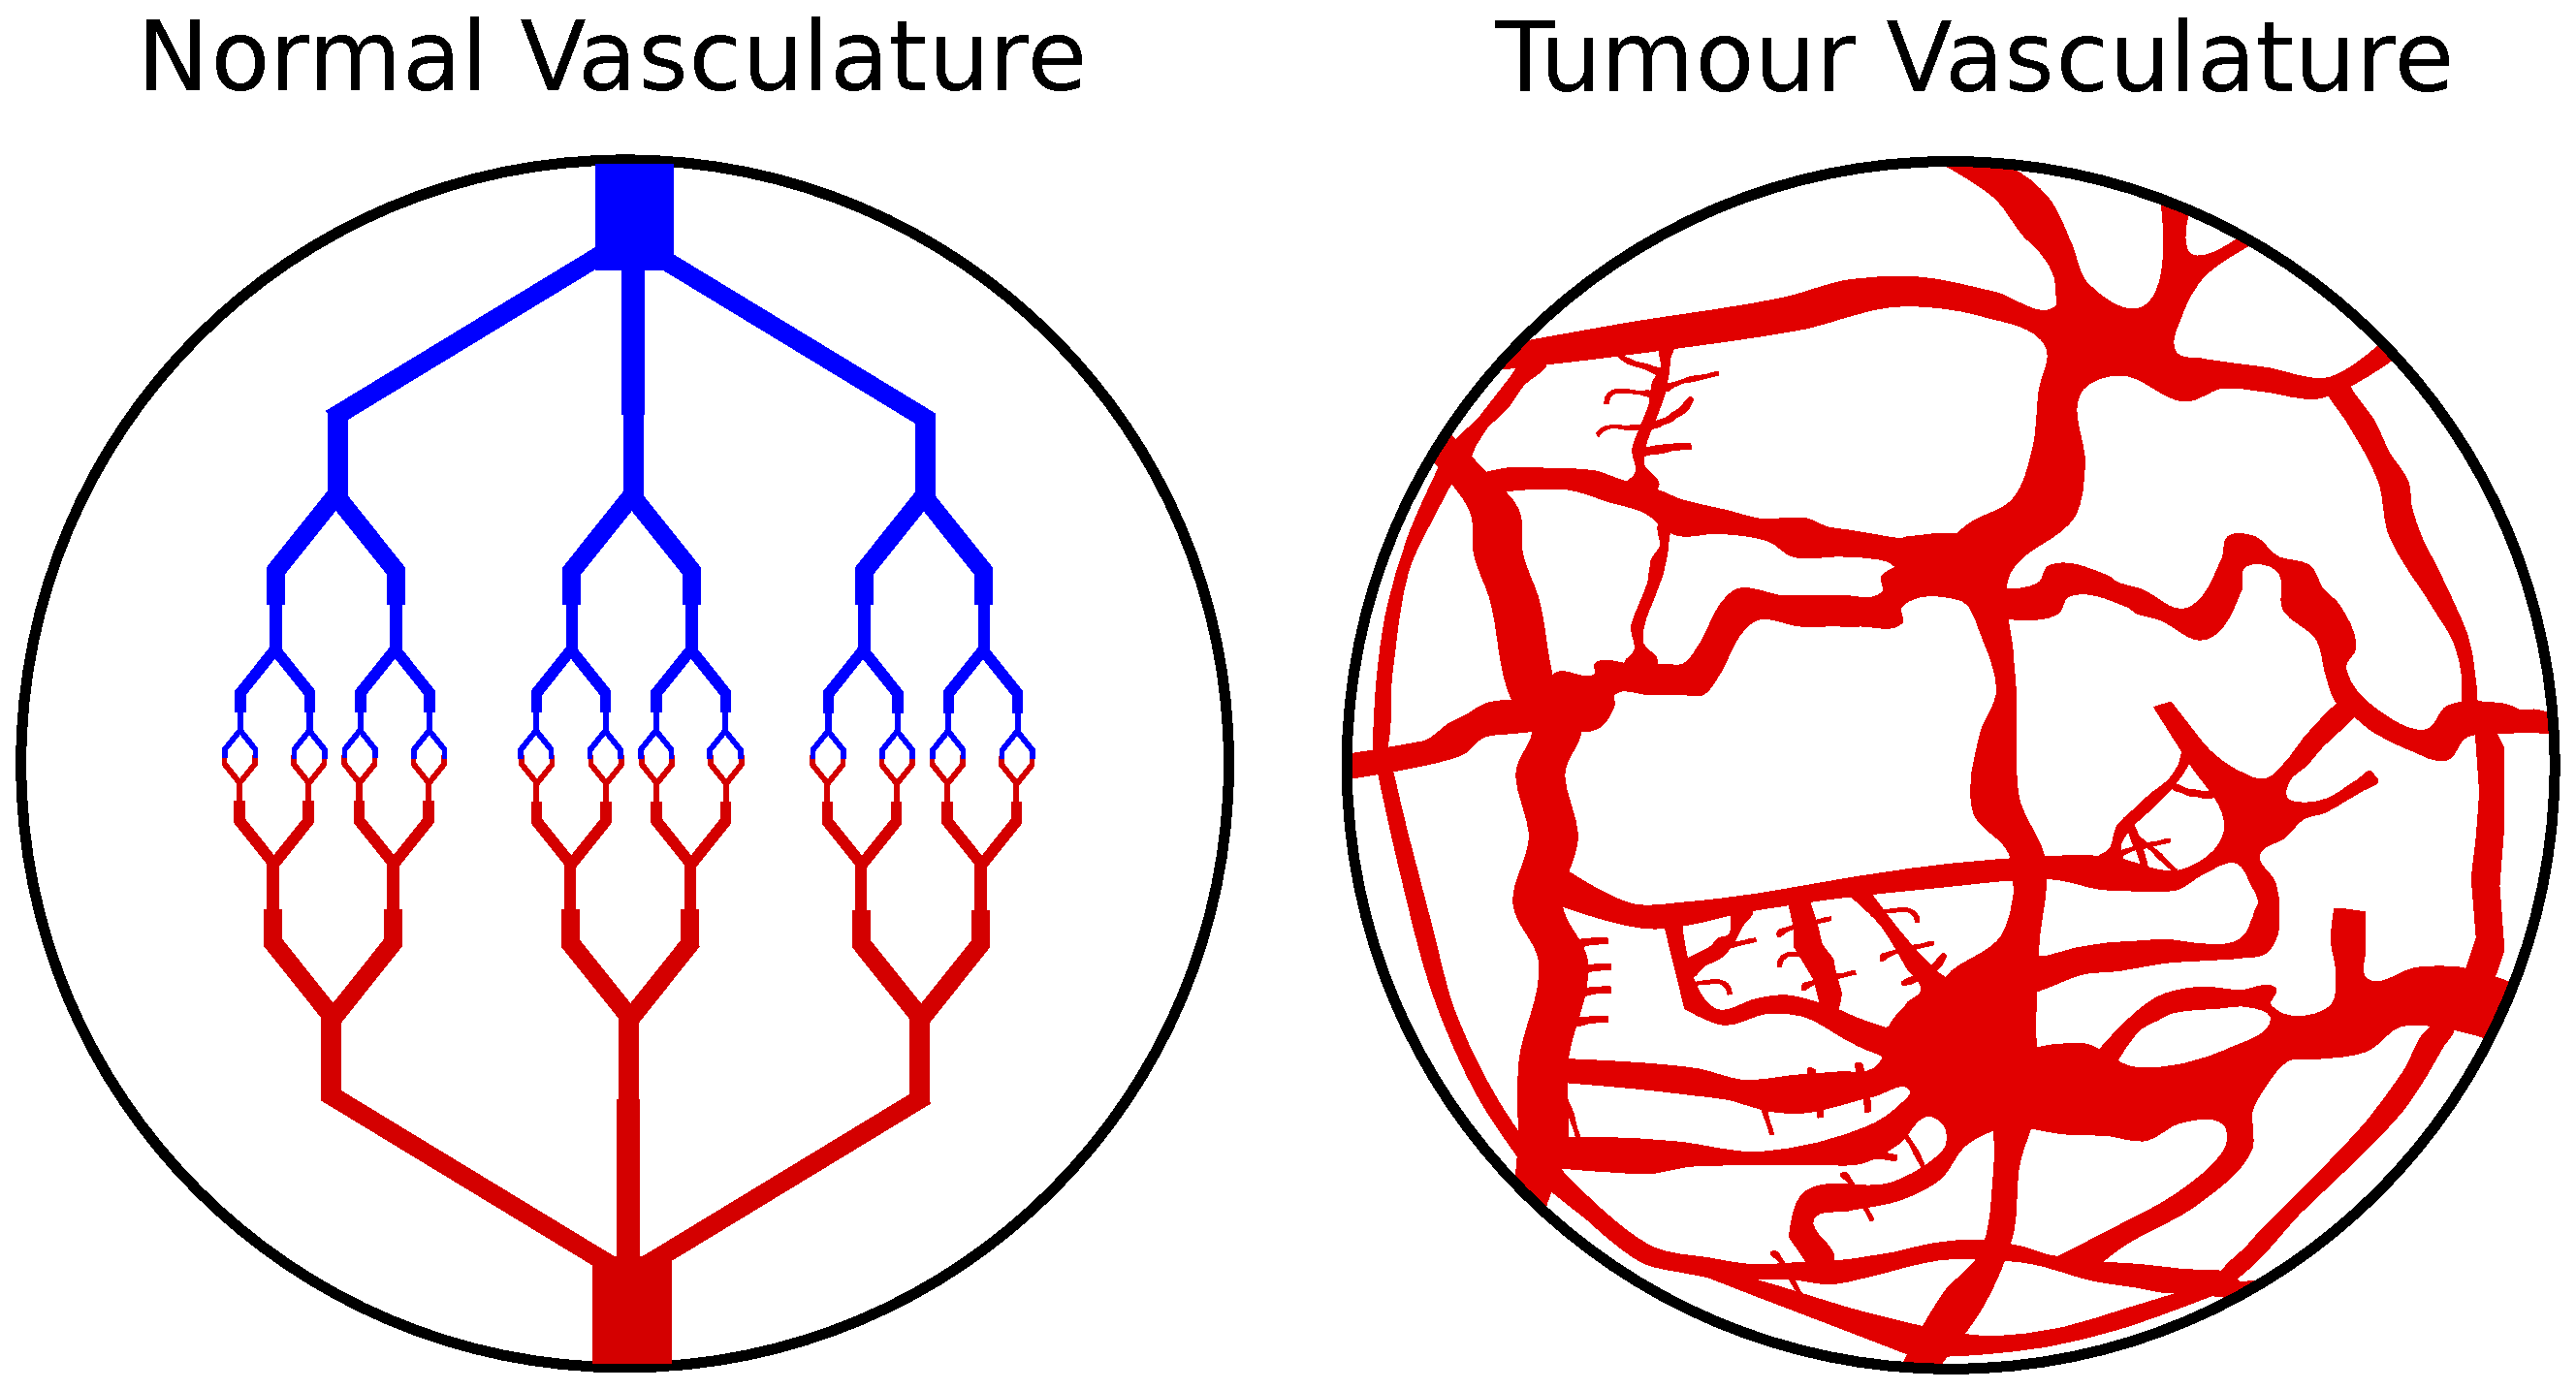
\includegraphics[width=4in]{intro/intro-images/tumourVasculature.pdf}
 \caption{Schematic of the normal tissue (left) and tumour (right) vasculature network. 
 Note the hierarchical structure of oxygenated blood (red) passing through the arteries, arterioles, and deoxygenated blood leaving via the venules, veins. 
 In tumours, this structure is severely compromised and often, no clear flow patterns can be distinguished with many vessels ending in dead ends or looping back onto feeding vessels.}
 \label{tumourVasculature}
 \end{center}
\end{figure}

%Several strategies have been proposed to maximize cell kill, including the combination of different therapies (such as radiotherapy and chemotherapy) and 
%Agents that ``normalize'' the tumour vasculature and prime them for receiving chemotherapies~\cite{Jain:2005gk}.
Tumour angiogenesis is extremely important in tumour growth, progression and metastasis and is a promising target for novel therapies~\cite{Miles:2000wq}.
For instance, measuring tumour angiogenesis has the potential to serve as a highly predictive prognostic marker for disease outcome and treatment.
Measurement of microvessel density using histology is generally considered an independent prognostic factor in several cancers~\cite{Kather:2015ej} but has several limitations.
Histology requires biopsy samples and patient comfort aside, biopsies only sample a small fraction of the affected organ.
The lack of functional information from biopsies as well as the practical challenges of obtaining longitudinal biopsy samples make non-invasive imaging a promising technique to complement and potentially reduce unneeded biopsies.
Angiogenesis is especially suitable for analysis with MRI due to its exquisite soft-tissue contrast, ability to image deep into the body, and finally its utility in assessing vascular function using injectable contrast agents.

\section{Animal models of cancer}

Developing models of human cancers in mice that predict clinical outcomes is beneficial as failure of novel chemotherapy drugs is often not determined until significant investments of time and money have been made designing and implementing phase I, II and III clinical trials~\cite{Rosenberg:1998ty}.
Animal models of cancer are essential for drug development, investigating mechanisms of action of physical phenomena, identifying gene targets, and protocol development prior to translating to human patients.
According to C$\acute{e}$spedes et al., an ideal cancer model should have the following characteristics~\cite{Cespedes:2006js}:
	
\begin{enumerate}
	\item Share histopathological features with the human tumour,
	\item Progress through the same stages and result in the same physiological and systemic effects,
	\item Share the same genes and biochemical pathways in both tumour initiation and tumour progression,
	\item Reflect the response of the human tumour to a particular therapy and
	\item Predict therapeutic efficacy in human clinical assays.
\end{enumerate}

Despite this, it is widely acknowledged that the translation potential of subcutaneous tumour xenograft models is limited particularly for translating chemotherapies to humans that have been shown effective in mice~\cite{Eklund:2013gm,deJong:2010cd}.
Naturally arising tumours often take years to months or years to grow but mouse xenograft models are selected so that experiments can be completed in days or weeks~\cite{Kamb:2005ix}.
The tumour vasculature that forms from injected tumour cells is fundamentally different from tumours that arise \emph{in vivo} as it lack the architectural and cellular complexity often seen in real tumours~\cite{Kamb:2005ix}.
Vessels in xenograft models typically grow much faster, are more chaotic in structure, have a leakier endothelium, and do not have much smooth muscle to regulate blood flow~\cite{Rosenberg:1998ty,Kamb:2005ix}. 

The heterogeneity of tumours also makes translation to humans difficult as within a specific tumour, several cell subpopulations exist that differ in their morphology, growth rate, receptor status and sensitivity to therapeutic potential~\cite{Hayes:2002ta,Heppner:1984ve}.
There are also regional differences in pH, degree of oxygenation, nutrient concentration that result in scattered pockets of hypoxia, apoptosis and necrosis  throughout the tumour~\cite{Hayes:2002ta, Jackson:2007uh,Heppner:1984ve}.
Vascular reorganization, particularly following treatment\cite{Wachsberger:2003vr,Kanthou:2002to}, leads to an irregular and shifting tumour microenvironment, a moving target for imaging modalities~\cite{Laking:2006ij}.
However, measuring these changes functionally, longitudinally, and non-invasively with imaging techniques has the potential to greatly improve our understanding of the tumour microenvironment.
Care must be taken not to over-interpret and generalize results from preclinical cancer studies.
Significantly more work needs to be done to obtain clinically relevant animal cancer models, but in the interim, animals models provide researchers with a valuable platform for developing novel agents of potential targets.

\section{Need for non-invasive imaging}
Non-invasive imaging methods are proving indispensable for studying angiogenesis \emph{in vivo} as they provide researchers with quantitative information about blood flow, vascular permeability, vessel density, vessel function and blood volume~\cite{McDonald:2003cm}.
Imaging modalities such as computed tomography (CT), magnetic resonance imaging (MRI), positron emission tomography (PET), single photon emission computed tomography (SPECT) and ultrasound (US), have all been proposed for studying angiogenesis~\cite{Laking:2006ij}.
Each modality is optimal for probing a particular aspect of biomarkers. 
To study angiogenesis and its effects on tumour growth and treatment response, the tumour environment needs to be probed using minimally invasive imaging techniques. 
Nuclear medicine techniques such as PET and SPECT employ radiotracers that can be measured at picomolar concentrations but at a significantly lower spatial resolution.
DCE-MRI and DCE-CT offer similar perfusion measurements (rate of leakage and leakage space) as both rely on the administration of a contrast agent that diffuses from the vasculature.
DCE-CT is advantageous as it has a direct linear relationship between the contrast agent concentration and the image intensity (attenuation numbers, given by Houndsfield Units)~\cite{Cuenod:2006jy}.
The disadvantage of CT however is that it requires ionizing radiation and iodinated contrast agents used in CT have been shown to have worse safety profiles compared to MR contrast agents~\cite{Hasebroock:2009hw}.
MRI can also be used to measure additional information such as diffusion, tissue oxygenation, spectroscopy, chemical exchange and magnetization transfer. 
In this thesis, several MRI techniques will be explored in a bid to improve our understanding of the tumour microenvironment.
We begin with some basic principles of MRI.

\section{Principles of Magnetic Resonance Imaging}

In biological specimens, water is by far the most abundant molecule in the body and the hydrogen atoms ($^{1}$H) in water are central to MR imaging.
Other MR-active nuclei include $^{13}$C, $^{19}$F, $^{23}$Na and $^{31}$P, but these are rare and not often used.
The molecular mass of a water molecule (H$_2$O) is approximately 18 g/mol and its density is 1 g/mL so in 1L, there are approximately 3$\times10^{25}$ molecules of water.
At the atomic level, each molecule of water consists of one oxygen atom (eight protons, neutrons, and electrons) as well as two hydrogen nuclei (a neutron and proton).
An intrinsic quantum mechanical property of fundamental particles such as the proton, neutron, and electron is that they posses angular momentum.
There are two types of angular momenta, spin and orbital angular momentum.
The proton and neutron possess only spin angular momentum but electrons also possess orbital angular momentum.
For electrons the two angular momenta nearly always cancel out in the lowest energy state of a chemically stable molecule such as water~\cite{Levitt:2001wo}.
The hydrogen nucleus has an odd number of protons (n=1) so there is a net spin angular momentum.
In fact, the only sources of angular momentum in the ground state are the molecular rotation and the nuclear spins associated with the proton and neutrons~\cite{Levitt:2001wo}.
Nearly all of the MR signal being measured in the body is derived from the hydrogen nuclei in water.

To summarize, each proton in the hydrogen nucleus has spin angular momentum, is charged and thus has a net magnetic moment.
Though there is no analogy to this from a classical physics perspective, one can imagine the net magnetic moment of a proton as a close cousin to the classical situation of the magnetic field generated by a loop of current in a wire.
We will model the hydrogen atom with a net magnetic moment as a small bar magnet spinning on its own axis (with an arrow vector representing the direction and strength of the magnetic moment) and rely on classical physics to describe the principle of magnetic resonance imaging. 
If a spinning bar magnet is placed in an external magnetic field, the magnetic moment vector of the bar magnet will precess, or rotate about the new magnetic field with a frequency known as the Larmor frequency:

\begin{equation}
	\vec{\mathbf{\omega}} = \gamma \vec{\mathbf{B_0}}
\end{equation}

The proportionality factor $\gamma$ is the gyromagnetic ratio and is nuclei-dependent and for protons, $\gamma = 42 MhZ /T$.
For convenience it is useful to change our reference frame to a rotating reference frame so the the magnetic moment vector is stationary on a (rotating) cartesian axis.

\begin{figure}
	\centering
	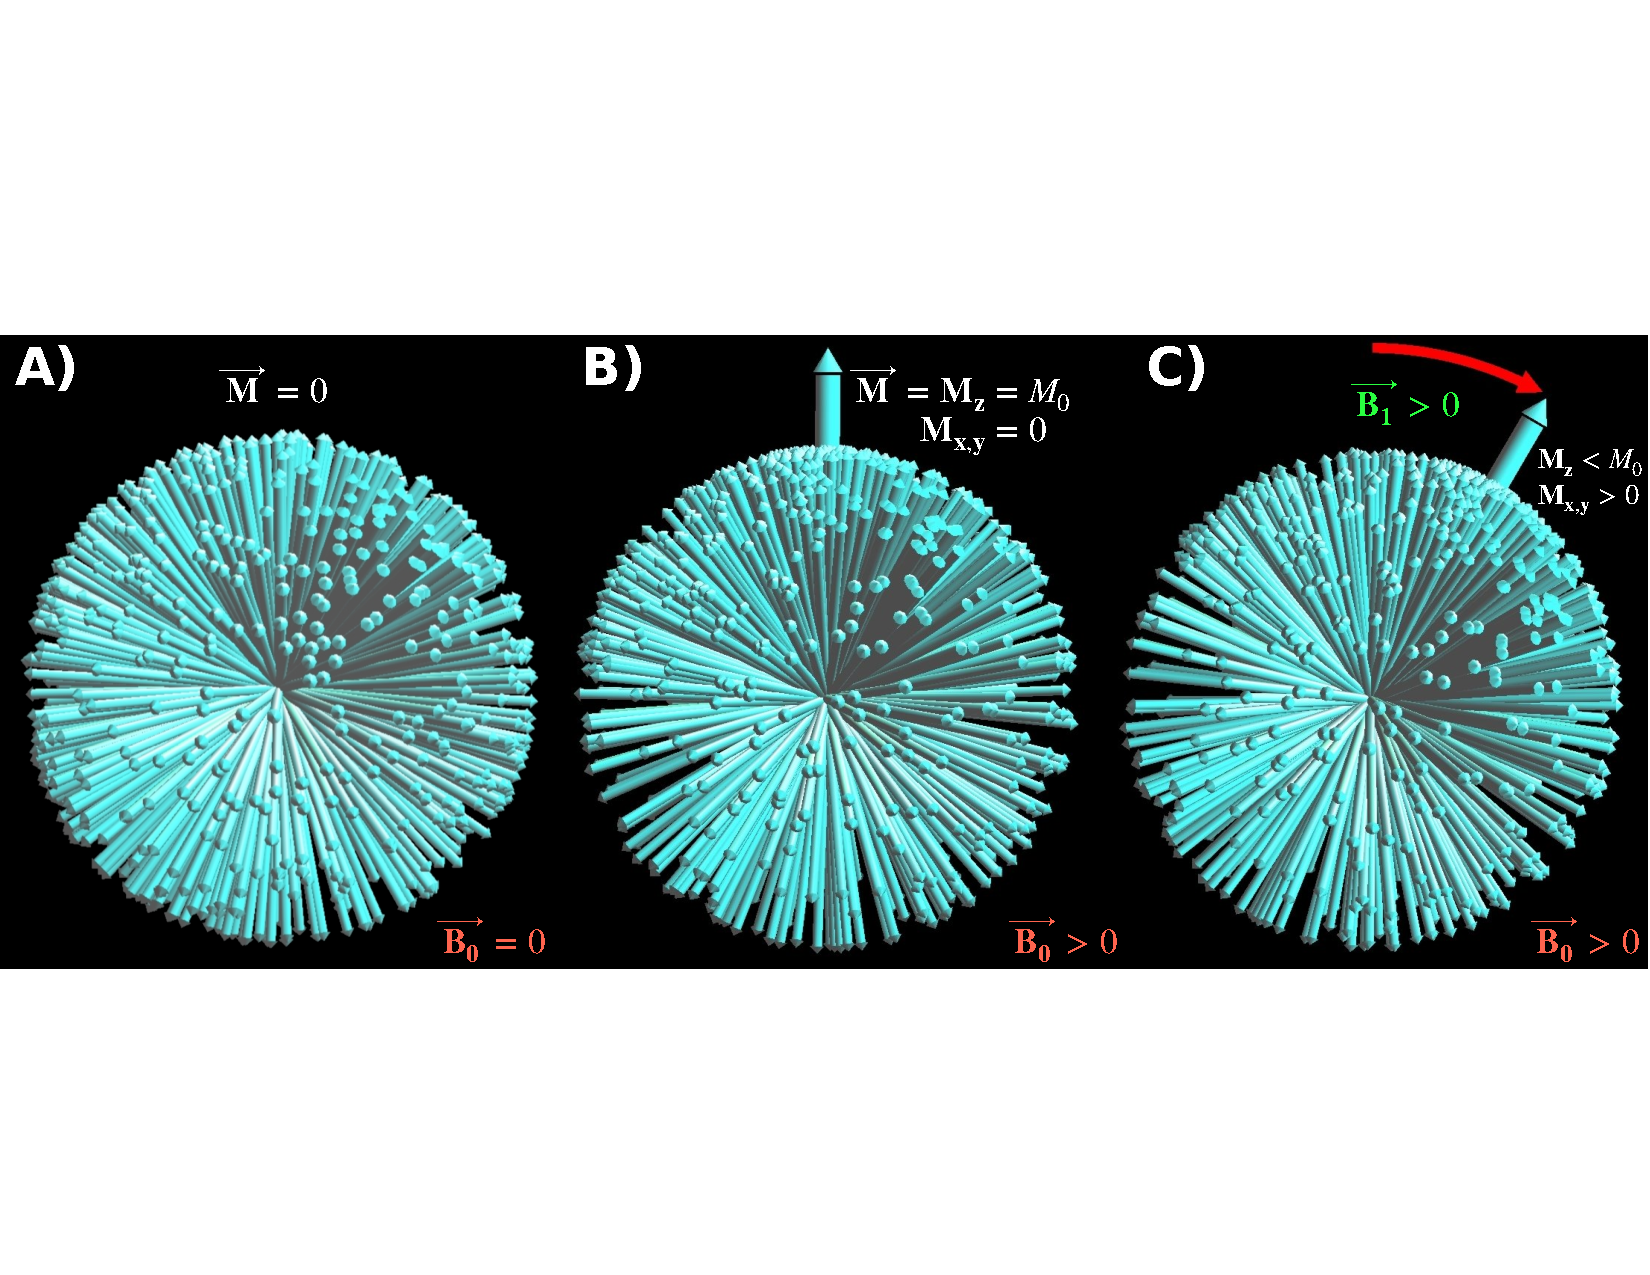
\includegraphics[width=\textwidth]{./intro/intro-images/HansonMRI.pdf}
	\caption{A) a collection of protons with magnetic moments are represented by arrows pointing in the direction of the magnetic moment, starting from a common starting point (centre). B) After switching on a main magnetic field $\vec{\mathbf{B_0}}$, the net magnetic moment $\vec{\mathbf{M}}$ slightly aligns with $\vec{\mathbf{B_0)}}$ because a larger fraction of spins point in the direction of the main magnetic field (in the rotating frame). C) The net magnetization moment is tipped to the transverse axis with an RF pulse $\vec{\mathbf{B_1}}$ so the signal can be measured. 
Annotations were added to the simulated images produced by Hanson et al.(\cite{Hanson:2008tp}), used with permission from Wiley and Sons.}
	\label{spinsB0B1}
\end{figure}

The quantity of interest in MRI is the net magnetic moment  $\vec{\mathbf{M}}$, and this is the summation of all individual magnetic moments present in the hydrogen nuclei. 
$\vec{\mathbf{M}}$ is the quantity that is measured and ultimately leads to the images produced.
Figure~\ref{spinsB0B1}A shows a schematic of the situation; for visualization, individual magnetic moments from the protons are localized to originate from the same central point.
Since the water molecules are tumbling around due to thermal motion, the proton magnetic moments are oriented randomly they are pointed in nearly every direction and there is no net magnetic moment (Fig.~\ref{spinsB0B1}A).
If we now put these water molecules into an MRI scanner and switch on a main magnetic field of strength $\vec{\mathbf{B_0}} = 7$ Tesla, there is a slight tendency of protons to align with the main magnetic field $\vec{\mathbf{B}}$ (along z axis, see Fig.~\ref{spinsB0B1}B), and a net magnetization vector $\vec{\mathbf{M}}$ is present.
$\vec{\mathbf{M}}$ aligns with $\vec{\mathbf{B_0}}$ and the longitudinal component $\mathbf{M_z} = M_0$ while the transverse component $\mathbf{M_{x,y}} = 0$ (in the x-y plane).
$\vec{\mathbf{M}}$ is many orders of magnitude smaller than the external magnetic field so the MR signal cannot be measured when it is aligned with the external main magnetic field $\vec{\mathbf{B_0)}}$. 
Applying a radiofrequency (RF) pulse $\vec{\mathbf{B_1}}$ at the Larmor frequency results in a torque applied to $\vec{\mathbf{M}}$, causing it to `tip' down into the transverse (x-y) plane (Fig.~\ref{spinsB0B1}C).

Interacting nuclei exchange energy with both the surrounding environment (spin-lattice interaction) as well as neighbouring nuclei (spin-spin interaction), and $\vec{\mathbf{M}}$ relaxes back to its equilibrium value. 
The time constant of the recovery of $\mathbf{M_z}$ to its equilibrium value $\vec{\mathbf{M_0}}$ is characterized by the time T$_1$,

\begin{equation}
	M_z = M_0(1-e^{-t/T_1})
	\label{T1}
\end{equation}

T$_1$ s after the RF pulse, the magnetization value has recovered to $\approx$ 63\% (1-e$^{-1}$) of its equilibrium value.
Prior to the $\vec{\mathbf{B_1}}$ pulse, the transverse component of the initial magnetization $\mathbf{M_{x,y}}$ was 0.
Following the $\vec{\mathbf{B_1}}$ pulse, $\mathbf{M_{x,y}}$ decays from its maximum value of $M_0$ to 0 through the interactions between nuclei and is characterized by the time constant T$_2$ (also called spin-spin relaxation).
		
\begin{equation}
		M_{xy} = M_0 e^{-t/T_2}
		\label{T2}
\end{equation}

Although T$_1$ and T$_2$ values are affected by various factors including field-strength, and local environmental factors such as temperature, proton concentration, and molecular mobility. 
Differences in T$_1$ and T$_2$ values are used to generate contrast between different tissues. 
For example, in a study conducted with ten volunteers at 1.5T, the spleen ($T_1 = 919$ ms), liver ($T_1 = 616$ ms), muscle ($T_1 = 785$ ms), fat ($T_1 = 239$ ms), and renal cortex ($T_1 = 919$ ms) all had measurably different $T_1$ values~\cite{OConnor:2009ku}.
Contrast between tissues can be generated by weighting images to highlight differences between T$_1$, T$_2$, and proton density.
In the next section, the sequence of choice for T$_1$-weighted images is described. 

\subsection{MRI sequences}

T$_1$-weighted images can be produced using both a spin echo pulse sequence as well as a gradient echo.
In a spin echo sequence, the magnetization is first flipped down to the transverse plane with a 90$^\circ$ RF pulse. 
Then the magnetization in the transverse plane is allowed to gradually de-phase and subsequently, a 180$^\circ$ RF pulse is applied causing the spins to re-phase.
Once the spins re-phase, an echo is produced and the time from the initial 90$^\circ$ to the eventual echo is the echo time, T$_E$. 
The 180$^\circ$ refocusing pulse is applied T$_E$/2 after the initial 90$^\circ$ pulse.
Specifying the T$_E$ allows control of image weighting - either T$_1$, T$_2$ or mixed weighted.
The repetition time T$_R$ is another important sequence parameter that controls how much magnetization, or signal is available to be flipped down to the transverse axis.
The repetition time is the time between subsequent 90$^\circ$ RF pulses - the longer the T$_R$, the more the longitudinal magnetization recovers and is available to be tipped down to the transverse plane at the next 90$^\circ$ RF pulse.

In a gradient echo sequence, only one RF pulse is needed to flip the magnetization to the transverse plane, and unlike the spin echo sequences, gradients are used to de-phase and re-phase the transverse magnetization.
The interpretation of T$_E$ is similar in a gradient echo and also measures the time between the 90$^\circ$ pulse and the echo produced after gradient re-phasing. 
Compared to the spin echo sequence, the use of gradients permits significantly shorter echo times and repetition times - T$_E$ and T$_R$ respectively.
This is why, in typical \acs{DCE-MRI} experiments, gradient echoes are preferred because signal acquisition is significantly faster allowing rapid and dynamic imaging.
To ensure there is no transverse magnetization after each repetition of the gradient echo sequence, spoiling is needed to suppress creation of spin and stimulated echoes.
The signal from a spoiled gradient echo (SPGR) sequence with spoiling and after steady state has been achieved is given by~\cite{Haase:2011fg}:

\begin{equation}
S=k\frac{\sin \alpha\left(1-e^{-T_R / T_1}\right)}{\left(1-(\cos \alpha) e^{-T_R / T_1}\right)} e^{-T_E / T_2^*}
\end{equation}

where $k$ is a proportionality constant that also includes the proton density.
In practice, if T$_E$ is small and close to T$_2^*$, this term (as it often is in SPGR sequences) approaches unity and is negligible. 
The signal characteristics of a spoiled gradient echo (SPGR) sequence is also shown in Figure~\ref{spgr_plot} with a specific T$_1$ of 2200 ms (typical T$_1$ values in tumours studied in this thesis) and with a T$_R$ of 120 ms.

The maximum signal intensity under these conditions is given by the Ernst angle, obtained by setting the derivative dS/d$\alpha$ = 0:

\begin{equation}
\alpha = arccos(e^{-T_R / T_1})
\end{equation}

\begin{figure}[htbp]
   \centering
   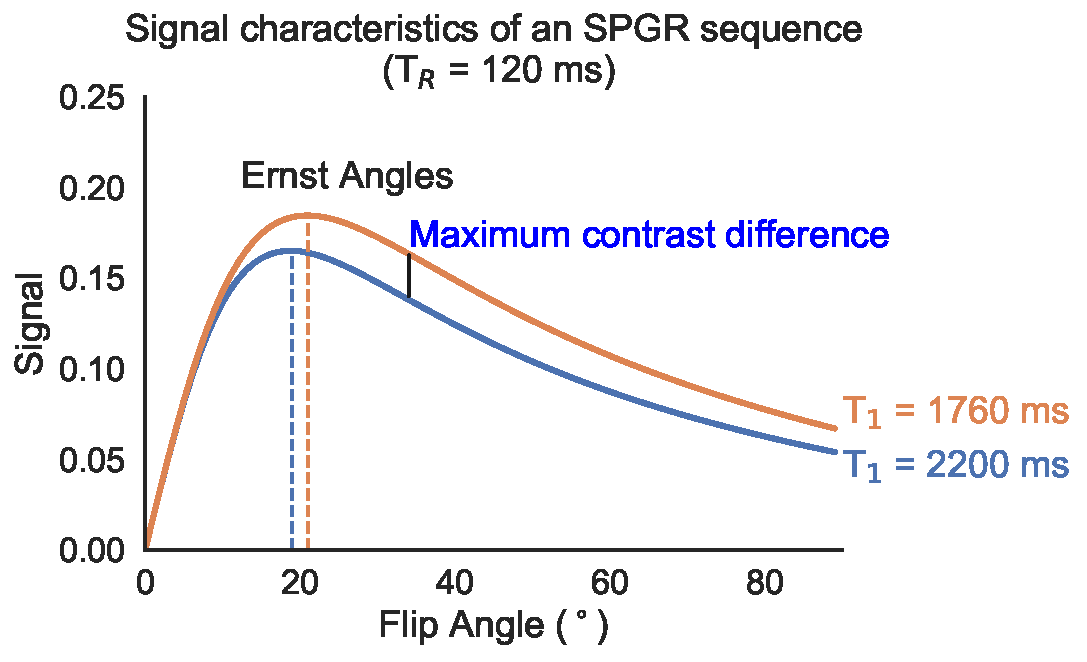
\includegraphics[width=\textwidth]{intro/intro-images/SPGR_plot.pdf}
   \caption{Dependence of flip angle on the signal from an SPGR sequence for two tissues with T$_1$ of 2200 and 1760 ms respectively. The Ernst angles for each tissue is marked with dotted lines, and the flip angle that would result in the maximum contrast difference is marked with a solid black line.}
   \label{spgr_plot}
\end{figure}

It is important to note that the Ernst angle maximizes the signal at a particular flip angle given a specific intrinsic T$_1$ but often it is necessary to optimize the signal difference between two (or more) species with different T$_1$ values.
The difference in signal intensities is the contrast ($\Delta$SI) between two tissue types. 
The maximum contrast difference for two tissues with T$_1$ values of 2200 and 1760 ms is marked with a solid black line in Fig.~\ref{spgr_plot}.
In Fig.~\ref{optimizing_TR}, the contrast ($\Delta$SI) and the T$_R$-normalized contrast ($\Delta$SI / $\sqrt{T_R}$) is shown as described by Busse~\cite{Busse:2005jt}.
From this figure - particularly the T$_R$-normalized contrast - we note that choice of T$_R$ is largely independent of optimizing contrast and there exists an optimal choice of flip angle regardless of the T$_R$.
This is important because very often, other factors such as SNR, temporal, and spatial resolution constrain the minimum T$_R$. 

\begin{figure}[htbp]
   \centering
   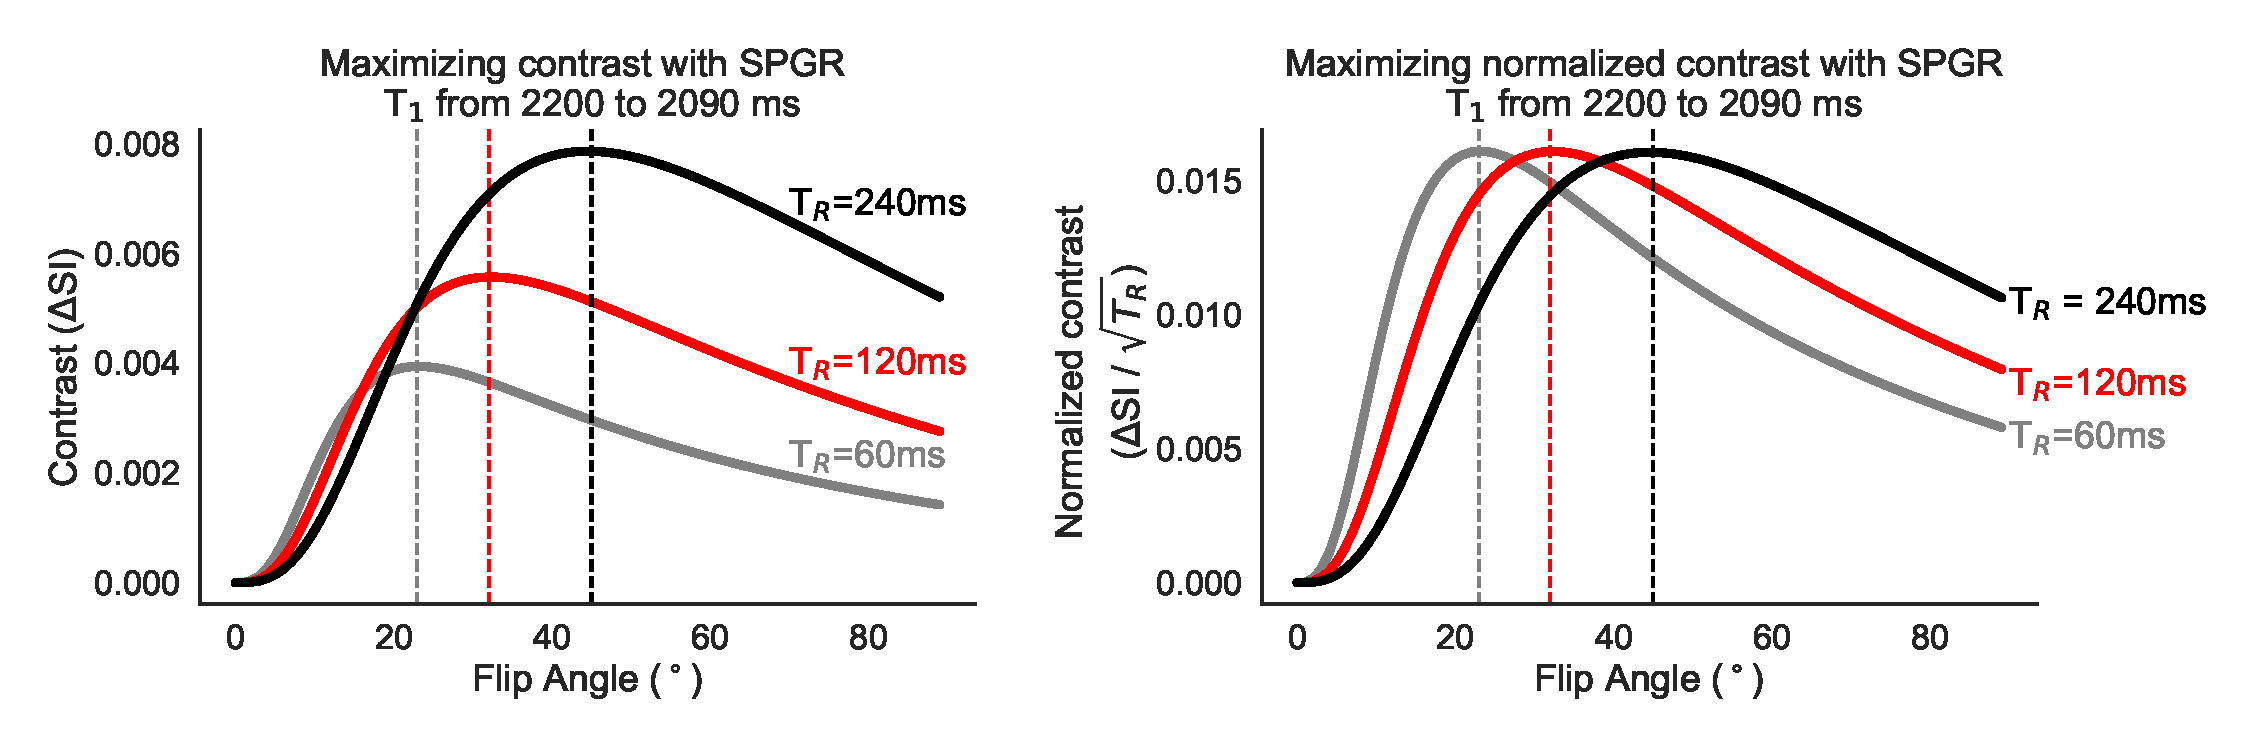
\includegraphics[width=\textwidth]{intro/intro-images/TR_FA_T1_optimization.pdf}
   \caption{On the left, the contrast ($\Delta$SI) for two tissues with T$_1$s of 2200ms and 2090ms for three T$_R$s are plotted along with the Ernst angles for each T$_R$. As the T$_R$ increases, the total available signal also increases because the magnetization has longer to recover. On the right, the curves are normalized by the T$_R$ which is more useful in optimizing sequence parameters. The three chosen repetition times (240ms in black, 120ms in red, and 60ms in grey) represent the range of T$_R$s used in the work presented in this thesis.}
   \label{optimizing_TR}
\end{figure}

For the sequences used in this thesis, competing factors were considered including imaging time, T$_1$-weighting, image intensity, SNR, image contrast, temporal, and spatial resolutions; appropriate compromises and trade-offs were made to balance the trade-offs to produce maximum benefit. 
Another tool at our disposal is the paramagnetic contrast agents as they are often used to increase the T$_1$ contrast between different species.
The following sections outline how dynamic contrast-enhanced MRI or \acs{DCE-MRI} is used in the imaging of cancer.

\subsection{Paramagnetic contrast agents}

Paramagnetism is defined as the intrinsic tendency for a material to become magnetized when placed within a magnetic field.
By far the most common element used as a contrast agent (tracer) in MRI is Gadolinium as it is strongly paramagnetic due to its seven unpaired electrons.
Because electrons are much smaller than protons but have the spins, they have a significantly higher gyromagnetic ratio.
The unbalanced electrons in the gadolinium shell or bonding orbital result in a strong net magnetic moment, which interacts with hydrogen nuclei and dramatically reduces the longitudinal relaxation time T$_1$ (and to a lesser extent T$_2$).
Unfortunately, free Gadolinium ions are toxic so they need to be attached to an organic chelating agent~\cite{DeLeonRodriguez:2015bl}.

The ability for a contrast agent to affect the T$_1$ relaxation time is given by its relaxivity $r_1$, obtained from the following equation:

\begin{equation}
\frac{1}{T_{1}} = \frac{1}{T_{1_0}} + r_1 [Gd]
\end{equation}

where T$_{1_o}$ is the initial T$_1$, prior to the influence of the paramagnetic contrast agent, $r_1$ is the relaxivity of the contrast agent in units of $(mM\cdot)^{-1}$, and $[Gd]$ is the contrast agent concentration.
It is important to note that all contrast agents shorten both T$_1$ and T$_2$ but whether their dominant influence is on the transverse relaxation time (T$_2$) or the longitudinal relaxation time (T$_1$) is expressed by the relative strengths of $r_1$ and $r_2$.

\subsection{Dynamic contrast-enhanced MRI (\acs{DCE-MRI})}

Through the use of a paramagnetic contrast agent, \acs{DCE-MRI} techniques increase contrast between species whose T$_1$ and T$_2$ times are otherwise very similar.
However the true value of \acs{DCE-MRI} comes from extracting physiologically relevant information from the body. 
In applications of cancer imaging, \acs{DCE-MRI} has been extremely successful in diagnostics, treatment monitoring, assessing severity of pathologies, distingushing between tumour models and types, improving our understanding of tumour metastases, and development of drugs.

Health Canada has approved eight gadolinium-based contrast agents for use in humans and they have molecular weights less than 1 \acs{kDa} that readily traverses the endothelium but not the cell membrane~\cite{WalkerSamuel:2006ch}. 
This property allows modelling of the vascular dynamics of the tumour but because the contrast agent is small, perfusion and permeability cannot be decoupled without extremely fast imaging and accurate knowledge of the arterial input function (\acs{AIF})\cite{Sourbron:2011ce}.
Choosing a kinetic model to fit the data requires some prior knowledge about the organ or system in question. 
For instance, the blood-brain barrier in the brain dramatically alters the contrast agent kinetics. 
Similarly, in leaky tumours the extravascular contrast agents typically used in \acs{DCE-MRI} leak out (and back in) of vasculature considerably faster than in other tissues. 
Sourbron et al.\ postulate that choice of a tracer kinetic model should provide a link between relevant physiological parameters and measured data~\cite{Sourbron:2011ce}. 

The most widely used model in \acs{DCE-MRI} is the extended Toft's model, which is valid in highly perfused tissues and weakly vascularized tissues with a well-mixed extravascular extracellular space ($v_e$)~\cite{Sourbron:2013jz}.
Figure~\ref{XTofts} provides a graphical description of this two compartment model, and its mathematical representation is:

\begin{equation}
C(t) = v_p \cdot AIF(t) + K^{trans}e^{-t\frac{K^{trans}}{v_e}} * AIF(t)
\end{equation}

where \acs{$v_p$} is the plasma volume, \acs{K$^{trans}$} is the volume transfer constant, and the $\acs{AIF}(t)$ is the arterial input function which needs to be measured independently of the contrast agent kinetics in the tissue.

\begin{figure}[htbp]
   \centering
   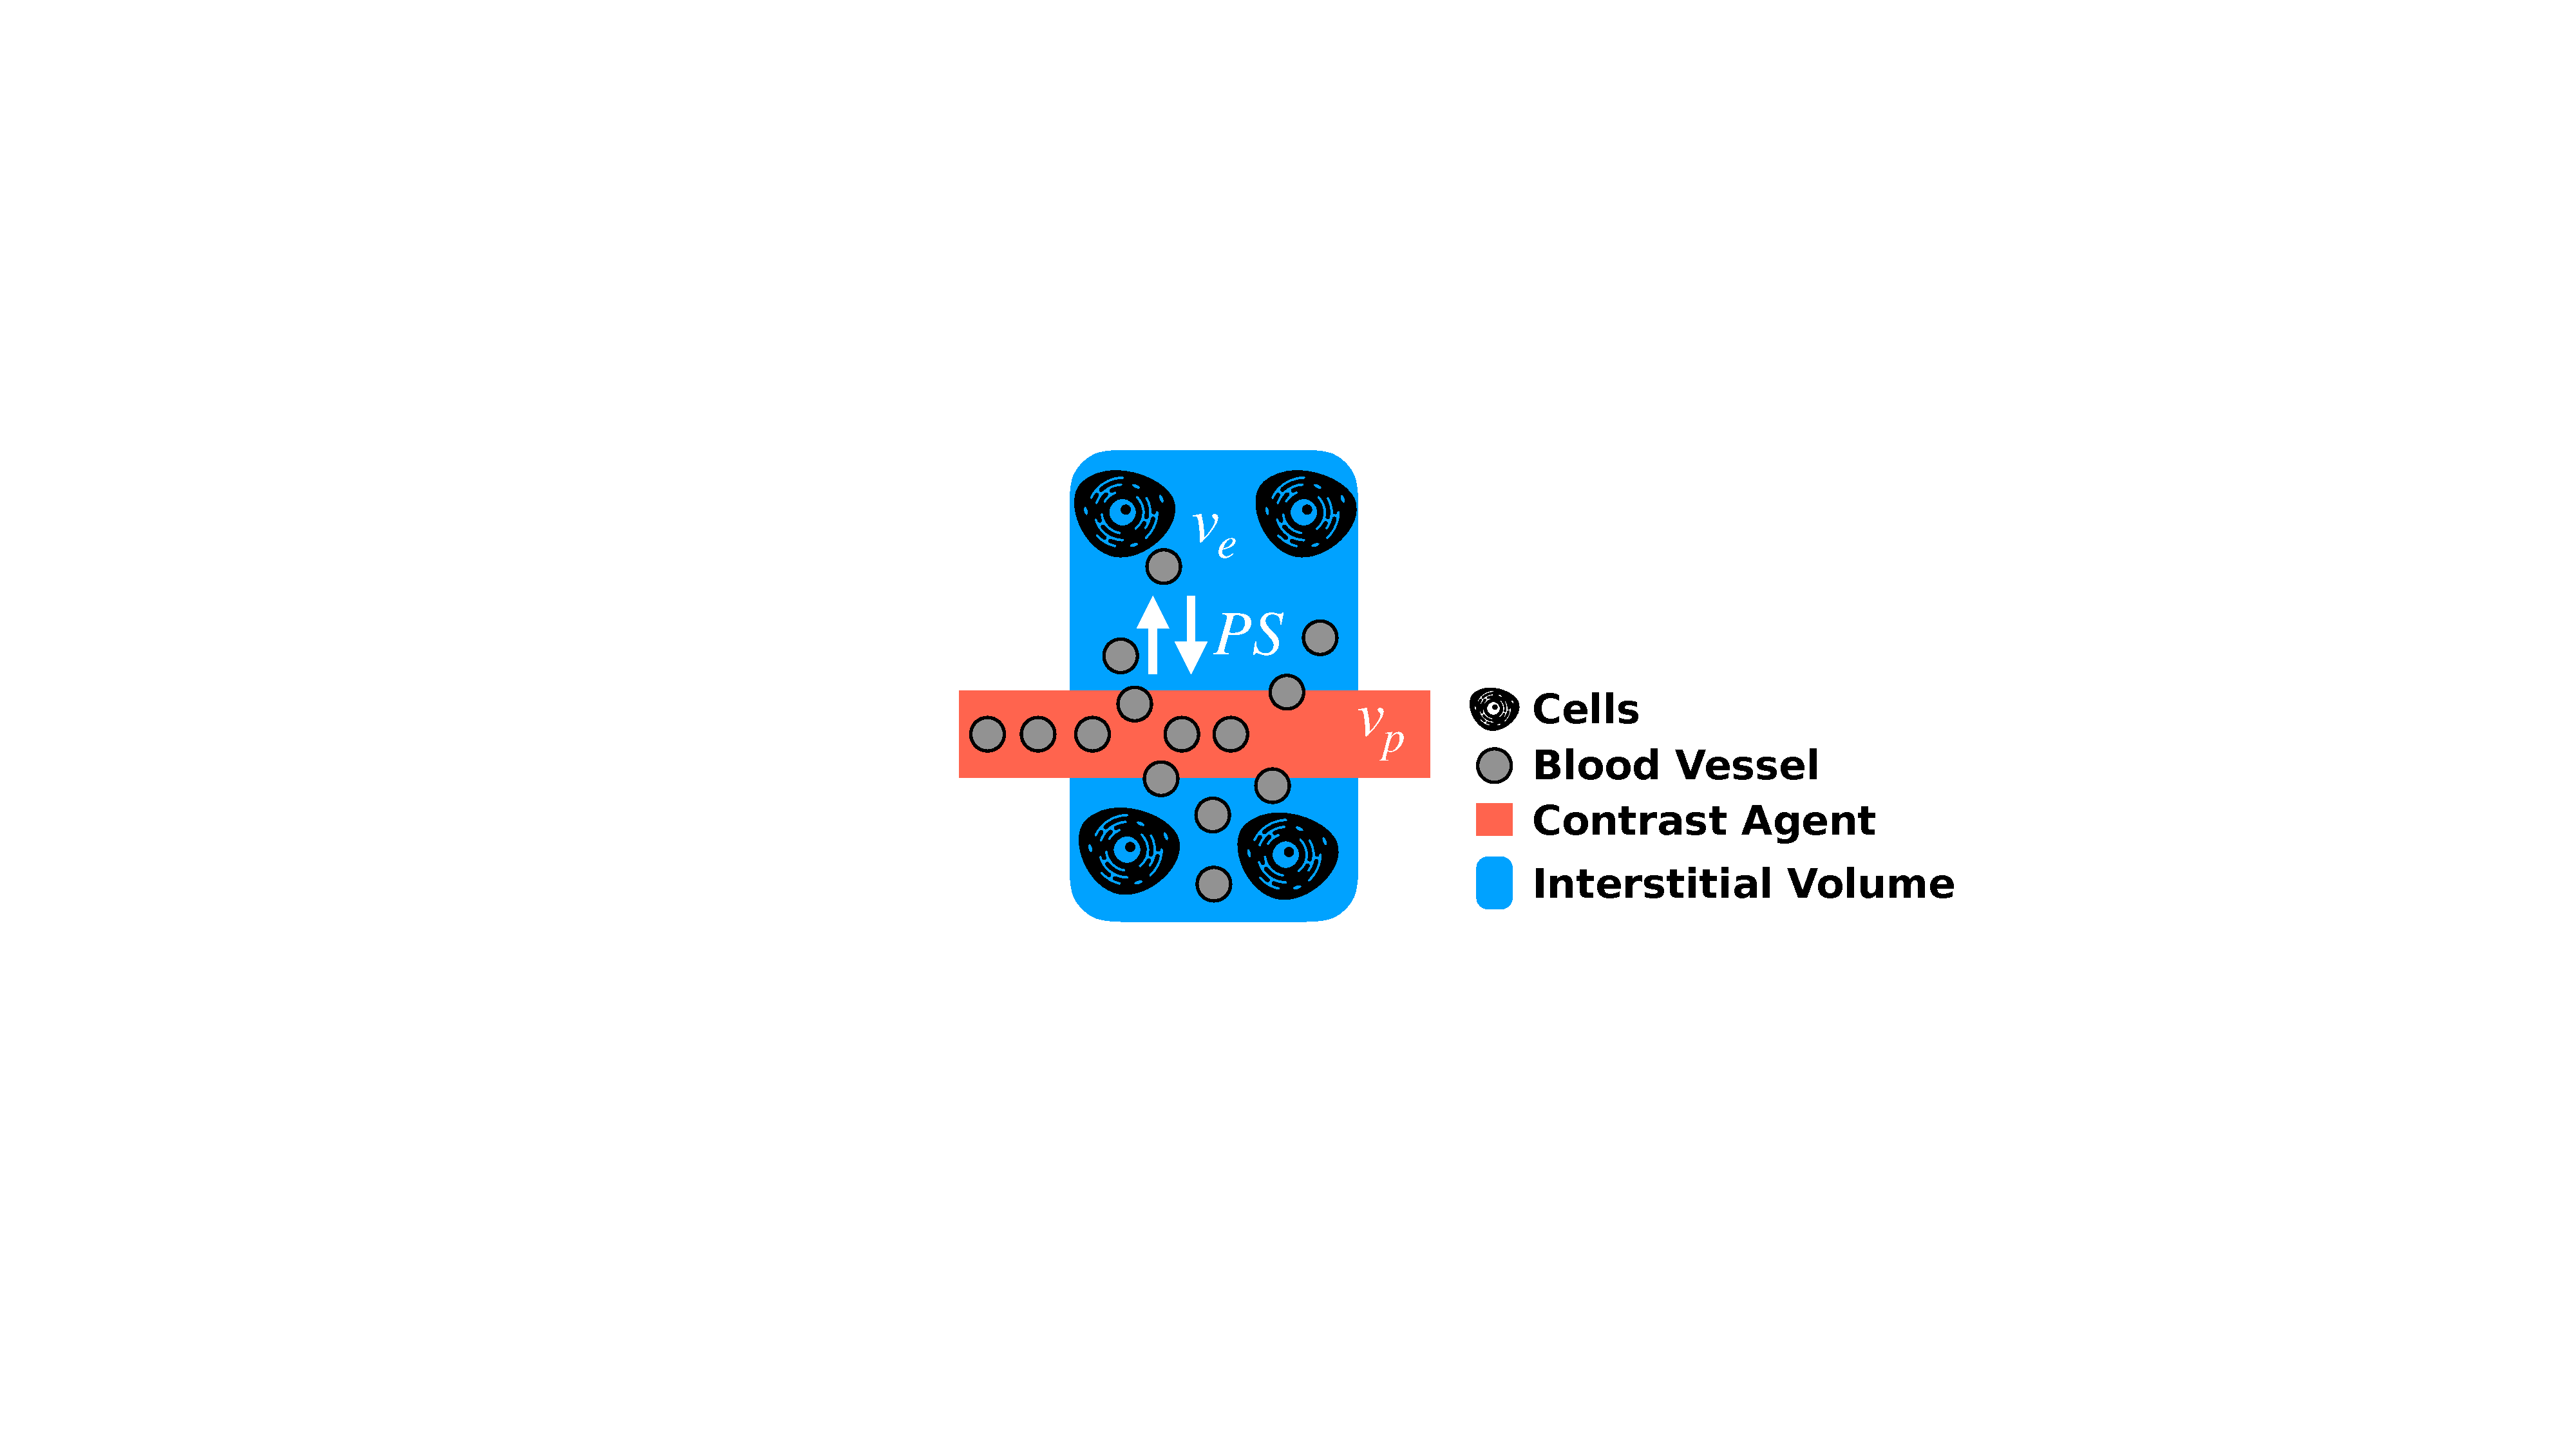
\includegraphics[width=\textwidth]{intro/intro-images/XTofts.pdf}
   \caption[Extended Tofts Model]{Graphical description of the Extended Tofts Model. An arterial input function (\acs{AIF}) governs the introduction of the tracer (grey circles) in the vascular compartment (pink) via a bolus injection. Contrast agent molecules exchanges with the extravascular extracellular space (\acs{$v_e$}, interstitial volume in blue) at a rate given by $PS$, the permeability-surface area product.}
   \label{XTofts}
\end{figure}

In this thesis, \acs{DCE-MRI} modelling using a traditional small molecule agent (\acs{Gd-DTPA} is used only briefly in Chapter~\ref{ch:HPG} and the \acs{AIF} used in that modelling was measured and published by a former lab member~\cite{Moroz:2013ee}.
Nevertheless, the concepts and introduction to \acs{DCE-MRI} are relevant for several portions of the thesis. 

\section{Thesis structure}

In \textbf{Chapter~\ref{ch:HPG}} a new macromolecular contrast agent is described and its value in describing the tumour microenvironment was explored.
A two-parameter linear model was applied to the contrast agent enhancement curve and measures of vessel permeability and fractional plasma volume were obtained.
These parameters were then used to distinguish between two tumour models.
In \textbf{Chapter~\ref{ch:HPG2}}, this technique was applied to determine whether molecule size played a role in the distribution of a high molecular weight anti-cancer drug (trastuzumab).
We showed that neither vessel permeability nor fractional plasma volume corresponded to presence of bound drug (determined via histological staining), indicating other barriers limit distribution of trastuzumab \emph{in vivo}.
In \textbf{Chapter~\ref{ch:HPG3}} we set out to determine whether our new contrast agent could assess changes in vessel permeability after treatment with an anti-angiogenic drug.
We discovered not only that vessel permeability is indeed reduced after treatment, but also that hypoxia dramatically decreased after treatment, as predicted by the vascular normalization hypothesis~\cite{Jain:2005gk}. 
This led us to develop a new method for assessing tumour oxygenation~\emph{in vivo} using MRI.
In \textbf{Chapter~\ref{ch:oemri1}}, we outlined how a blind source separation technique increased the sensitivity of existing methods. 
The technique was validated in \textbf{Chapter~\ref{ch:oemri2}} with histological staining, and we demonstrated utility of a new parameter to separate oxygenation replenishment in different tumour models.
Finally in \textbf{Chapter~\ref{ch:oemri3}} we showcase a typical application of the technique: detection of tumour oxygenation improvements after administering an anti-angiogenic agent. 
We also showed that the tumour implant site has a large bearing on the tumour microenvironment, and no oxygenation improvements are observed if the baseline oxygenation is high.
In \textbf{Chapter~\ref{ch:futurework}}, interesting observations are presented that may be useful starting points for future work in this field.